%% genome_feature_comparisons.tex
%% Author: Leighton Pritchard
%% Copyright: James Hutton Institute
%% Genome feature comparisons

%
\begin{frame}
  \frametitle{Gene features}
  Significant substructure, especially in eukaryotes
  \begin{columns}[T] 
    \column{.4\textwidth} 
      \begin{itemize}
        \item translation start
        \item introns
        \item exons
        \item translation stop
        \item translation terminator
      \end{itemize}
    \column{.6\textwidth}
      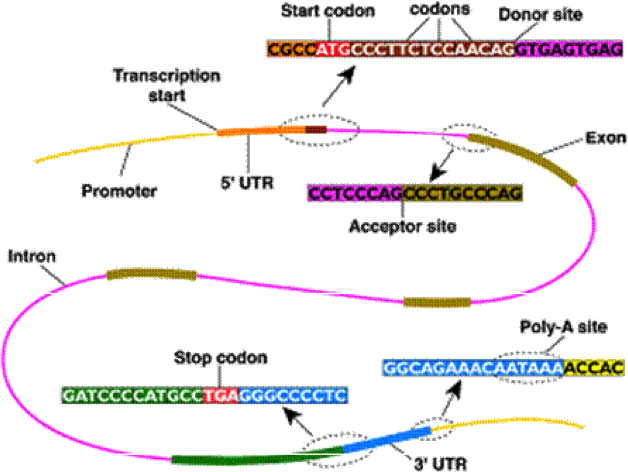
\includegraphics[width=\textwidth]{images/gene_feature}
  \end{columns}    
\end{frame}

%
\begin{frame}
  \frametitle{RNA features}
  \textcolor{hutton_blue}{RNA/ncRNA: characterised by complex secondary structure}
  \begin{columns}[T] 
    \column{.4\textwidth} 
      \begin{itemize}
        \item tRNA - transfer RNA
        \item rRNA - ribosomal RNA
        \item CRISPRs - prokaryotic defence, and genome editing
        \item many other functional classes, including enhancers
      \end{itemize}
    \column{.6\textwidth}
      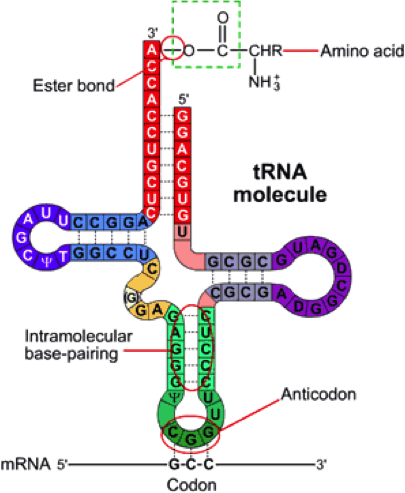
\includegraphics[height=0.7\textheight]{images/rna_feature}
  \end{columns}    
\end{frame}

%
\begin{frame}
  \frametitle{Regulatory features
  \footnote{\tiny{\href{http://dx.doi.org/10.1038/35052548
}{Pennacchio \& Rubin (2001) \textit{Nature Rev. Genet.} doi:10.1038/35052548
}}}  
  }
  \begin{itemize}
    \item transcription start sites (TSS)
    \item RNA polymerase (RNAp) binding sites
    \item transcription factor binding sites (TFBS)
    \item core, proximal and distal promoter regions
  \end{itemize}
  \begin{center}
    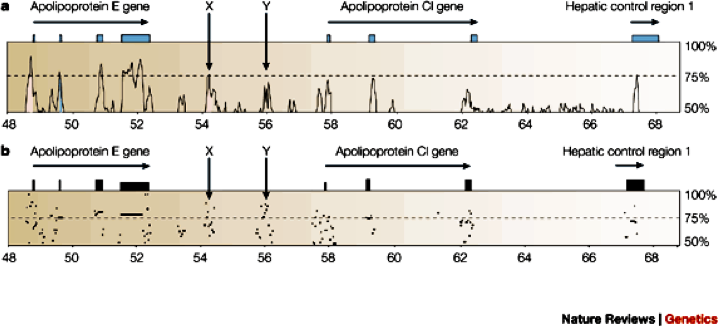
\includegraphics[width=0.8\textwidth]{images/regulatory_feature} \\
    \textcolor{hutton_green}{human vs mouse comparison}
  \end{center}    
\end{frame}

%
\begin{frame}
  \frametitle{Gene finding
  \footnote{\tiny{\href{http://dx.doi.org/10.1101/gr.088997.108
}{Liang \textit{et al.} (2009) \textit{Genome Res.} doi:10.1101/gr.088997.108
}}}
    \footnote{\tiny{\href{http://dx.doi.org/10.1038/nbt0807-883
}{Brent (2007) \textit{Nat. Biotech.} doi:10.1038/nbt0807-883
}}}
    \footnote{\tiny{\href{http://dx.doi.org/10.1186/1471-2105-5-59
}{Korf (2004) \textit{BMC Bioinf.} doi:10.1186/1471-2105-5-59
}}}
    }
  At genome scales, we need to automate functional prediction \\~\\    
  \textcolor{hutton_green}{Empirical (evidence-based) methods:}
  \begin{itemize}
    \item Inference from known protein/cDNA/mRNA/EST sequence
    \item Interference from mapped RNA reads (e.g. RNAseq)
  \end{itemize}
  \textcolor{hutton_blue}{\textit{Ab initio} methods:}
  \begin{itemize}
    \item Prediction on the basis of gene features (TSS, CpG islands, Shine-Dalgarno sequence, stop codons, nucleotide composition, etc.)
  \end{itemize}
  \textcolor{hutton_purple}{\textbf{Inference from genome comparisons/sequence conservation}}
\end{frame}

%
\begin{frame}
  \frametitle{Regulatory element finding
  \footnote{\tiny{\href{http://dx.doi.org/10.1186/1471-2105-12-238
}{Zhang \textit{et al.} (2011) \textit{BMC Bioinf.} doi:10.1186/1471-2105-12-238
}}}
    \footnote{\tiny{\href{http://dx.doi.org/10.1093/nar/gkt1123
}{Kilic \textit{et al.} (2013) \textit{Nucl. Acids Re.} doi:10.1093/nar/gkt1123
}}}
    \footnote{\tiny{\href{http://dx.doi.org/10.1016/j.gde.2005.05.002
}{Vavouri \& Elgar (2005) \textit{Curr. Op. Genet. Deve.} doi:10.1016/j.gde.2005.05.002
}}}
    }
  \textcolor{hutton_green}{Empirical (evidence-based) methods:}
  \begin{itemize}
    \item Inference from protein-DNA binding experiments
    \item Interference from co-expression
  \end{itemize}
  \textcolor{hutton_blue}{\textit{Ab initio} methods:}
  \begin{itemize}
    \item Identification of regulatory motifs (profile/other methods; TATA, $\sigma$-factor binding sites, etc.)
    \item Statistical overrepresentation of motifs
    \item Identification from sequence properties
  \end{itemize}
  \textcolor{hutton_purple}{\textbf{Inference from genome comparisons/sequence conservation}}
\end{frame}

% What do you align, and why?
\begin{frame}
  \frametitle{Equivalent genome features}
  \begin{center}
    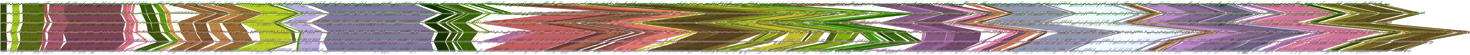
\includegraphics[width=1\textwidth]{images/collinear_zeae}  
  \end{center}
  When comparing two features (e.g. genes) between two or more genomes, there must be some basis for making the comparison. \\
  \textcolor{hutton_blue}{They have to be \textit{equivalent} in some way, such as:}
  \begin{itemize}
    \item common evolutionary origin
    \item functional similarity
    \item a family-based relationship
  \end{itemize}
  \textcolor{hutton_purple}{It's common to define equivalence of genome features in terms of evolutionary relationship.}
\end{frame}

% What do you align, and why?
\begin{frame}
  \frametitle{Why look at equivalent features?}
  \begin{center}
    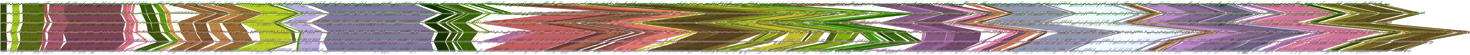
\includegraphics[width=1\textwidth]{images/collinear_zeae}  
  \end{center}
  \textbf{The real power of genomics is comparative genomics!}
  \begin{itemize}
    \item Makes catalogues of genome components comparable between organisms
    \item \textcolor{hutton_blue}{Differences, e.g. presence/absence of equivalents may support hypotheses for functional or phenotypic difference}
    \item \textcolor{hutton_green}{Can identify characteristic signals for diagnosis/epidemiology}
    \item \textcolor{hutton_purple}{Can build parts lists and wiring diagrams for systems and synthetic biology}
  \end{itemize}
\end{frame}

%
\begin{frame}
  \frametitle{Who let the -logues out?}
  \Large{
    \textcolor{olive}{
      \textbf{
      Genome features can have complex evolutionary relationships \\~\\
      We have precise terms to describe these relationships
      }
    }
  }
  \begin{center}
    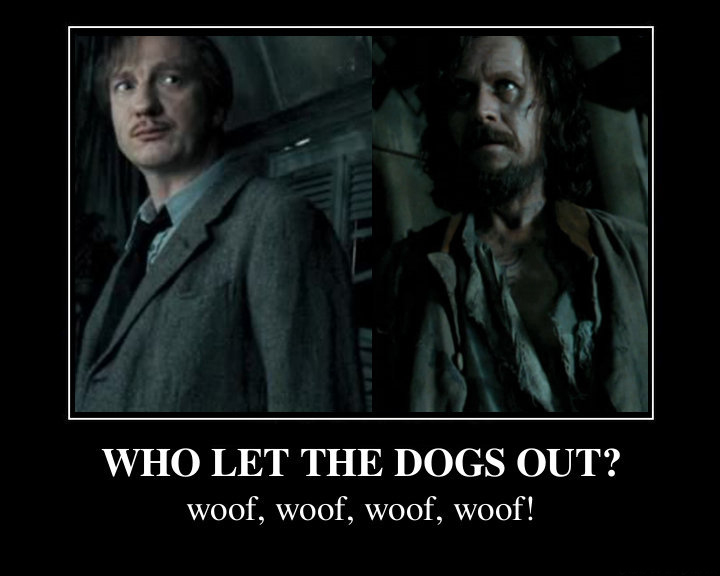
\includegraphics[width=0.4\textwidth]{images/who_let_the_dogs_out}
  \end{center}      
\end{frame}

%
\begin{frame}
  \frametitle{The -logues drop
  \footnote{\tiny{\href{http://dx.doi.org/10.2307/2412448
}{Fitch \textit{et al.} (1970) \textit{Syst. Zool.} doi:10.2307/2412448
}}}
  }
  How do we understand the relationships between features in more than one genome?
  \begin{itemize}
    \item \textcolor{hutton_green}{Functional similarity}: \textbf{analogy}
    \item \textcolor{hutton_blue}{Evolutionary common origin}: \textbf{homology, orthology, etc.}
    \item \textcolor{hutton_purple}{Evolutionary/functional/family relationship}: \textbf{paralogy}
  \end{itemize}
  \begin{center}
    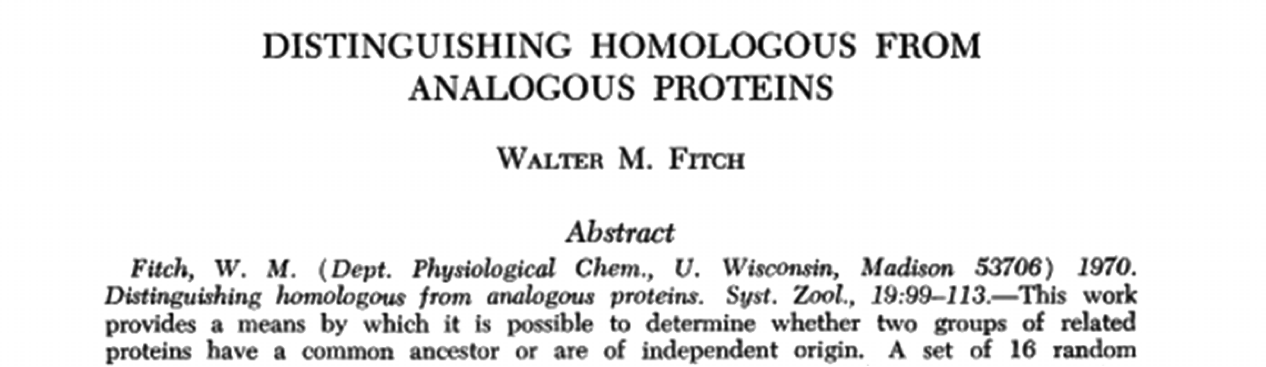
\includegraphics[width=\textwidth]{images/fitch}
  \end{center}    
\end{frame}

% 
\begin{frame}
  \frametitle{Who let the -logues out?}
  \begin{center}
    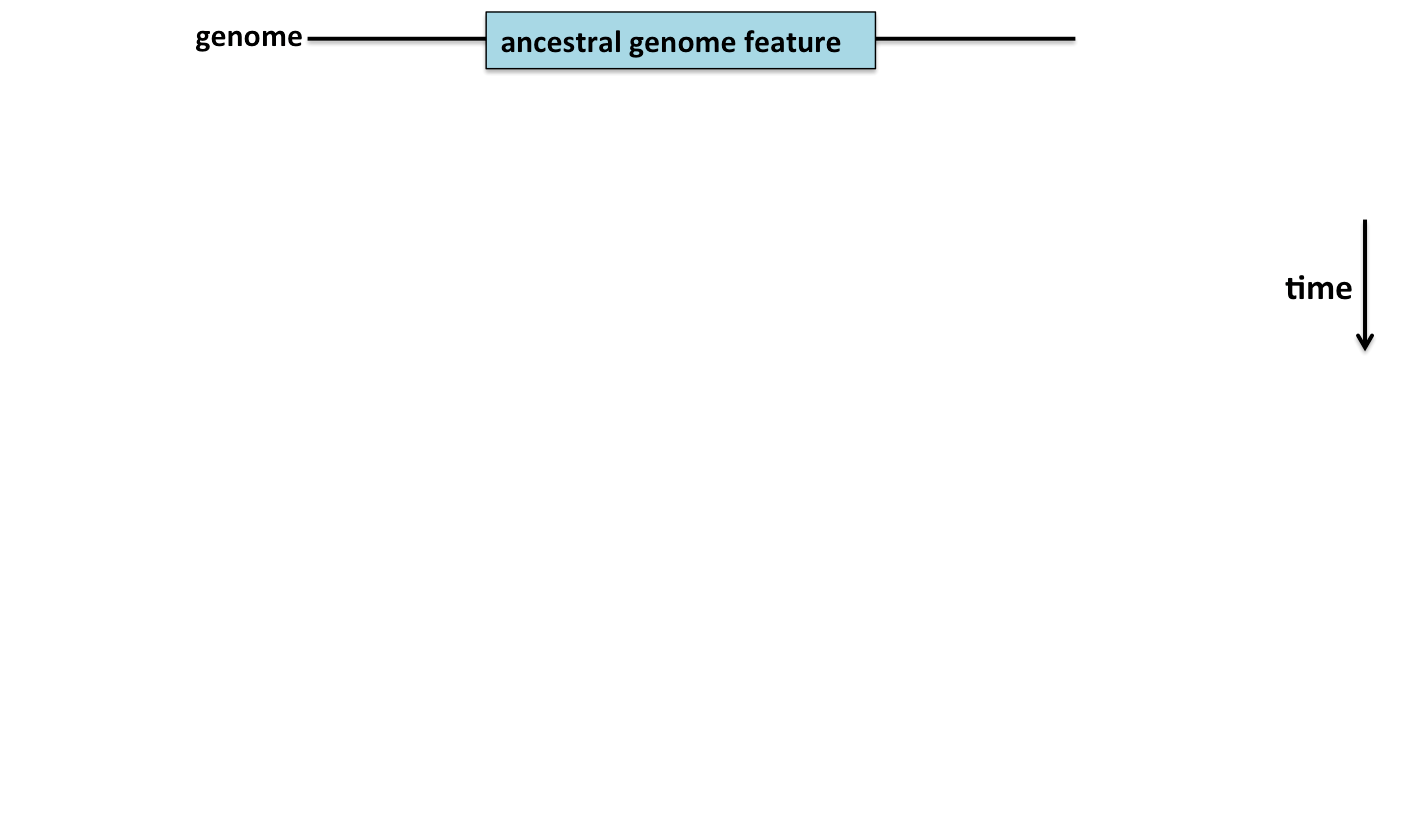
\includegraphics[width=1\textwidth]{images/logues1}  
  \end{center}  
\end{frame}

% 
\begin{frame}
  \frametitle{Who let the -logues out?}
  \begin{center}
    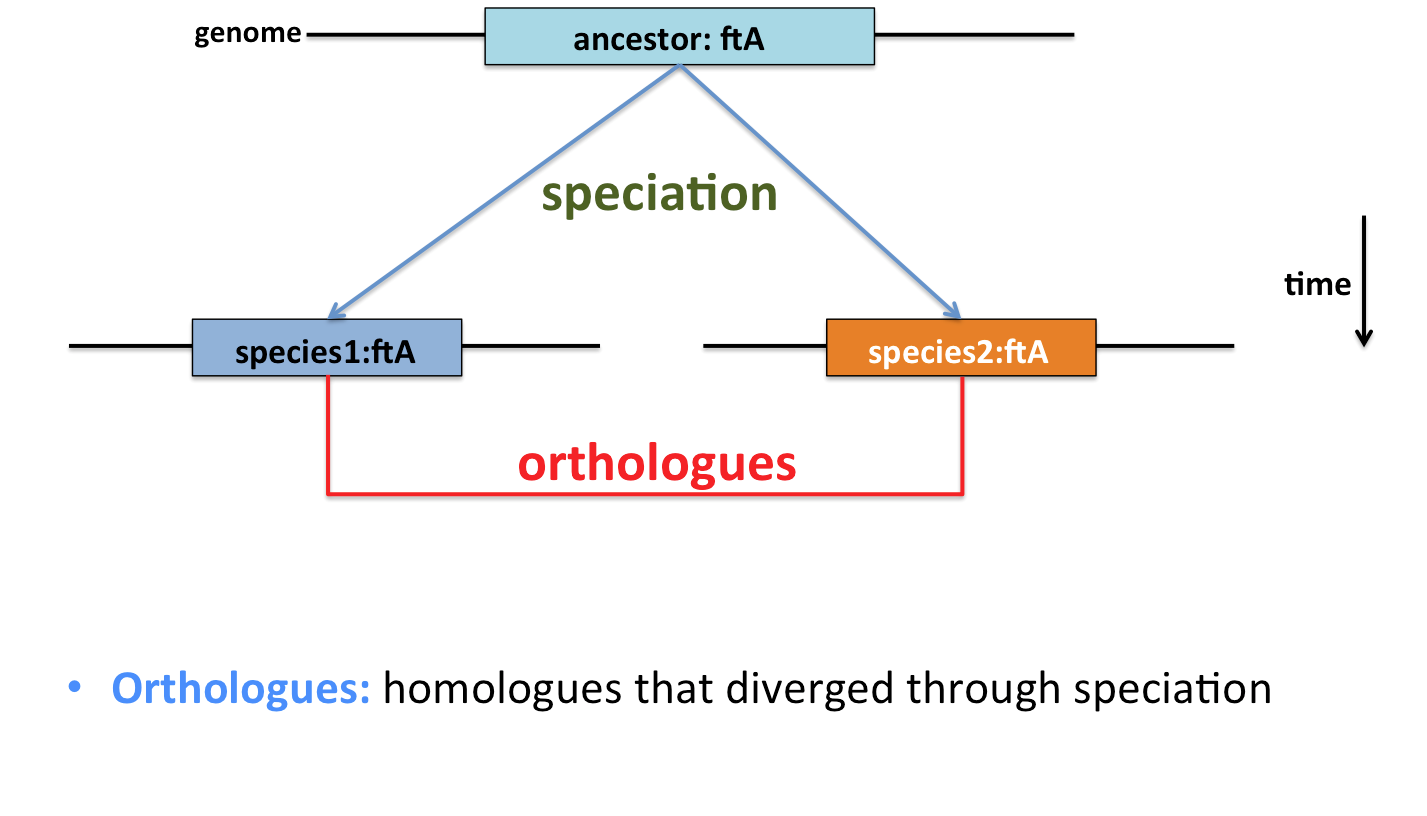
\includegraphics[width=1\textwidth]{images/logues2}  
  \end{center}  
\end{frame}

% 
\begin{frame}
  \frametitle{Who let the -logues out?}
  \begin{center}
    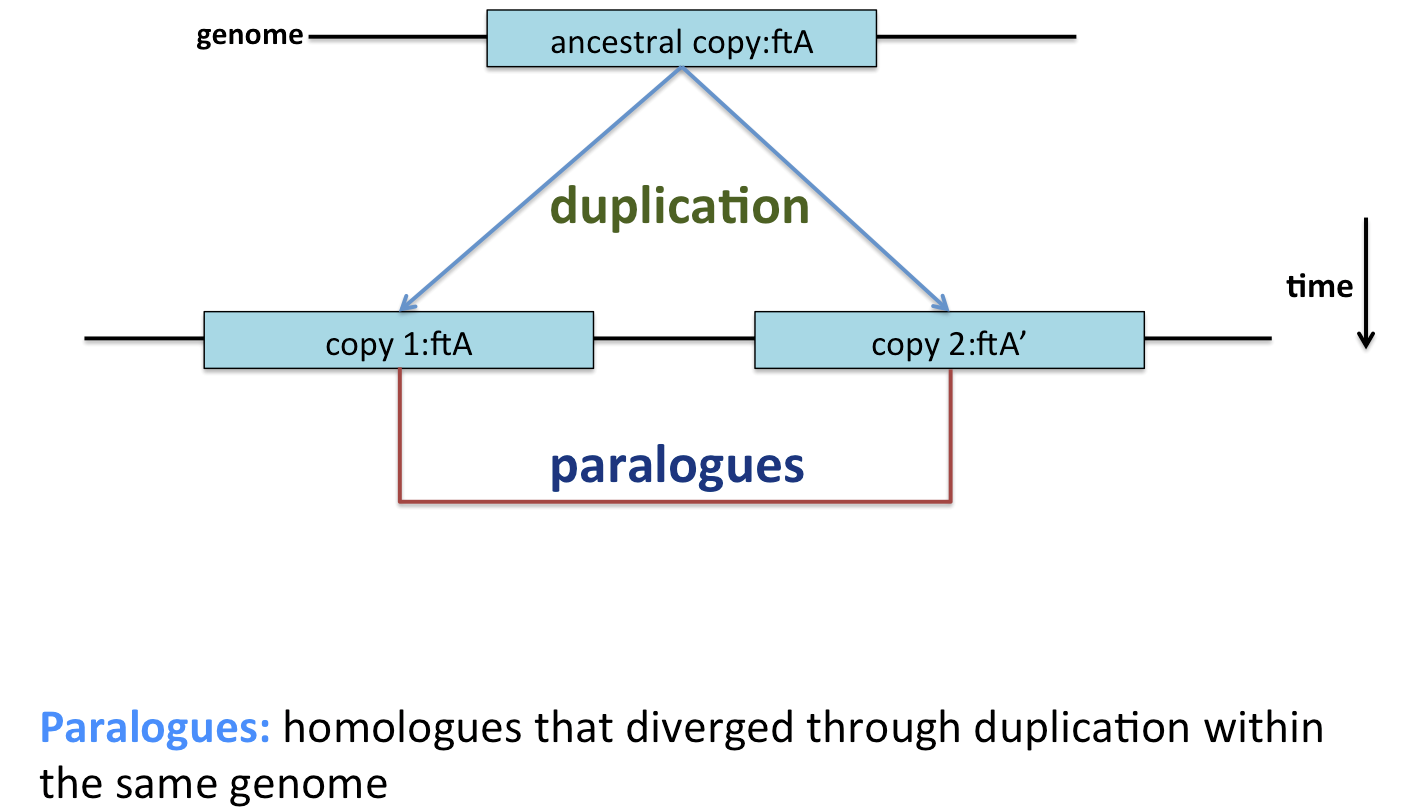
\includegraphics[width=1\textwidth]{images/logues3}  
  \end{center}  
\end{frame}

% 
\begin{frame}
  \frametitle{Orthology
    \footnote{\tiny{Storm \& Sonnhammer (2002) \textit{Bioinformatics} \href{http://dx.doi.org/10.1093/bioinformatics/18.1.92}{doi:10.1093/bioinformatics/18.1.92
    }}}
    }
  \begin{itemize}
    \item \textcolor{RawSienna}{Frequently abused/misused as a term}
    \item \textcolor{hutton_green}{``Orthology'' is an evolutionary relationship, bent into service as a functional descriptor}
    \item \textcolor{hutton_blue}{Orthology is strictly defined \textit{only for two species or clades}! (cf. OrthoMCL)}
    \item \textcolor{hutton_purple}{Orthology is not transitive: \\ ($A$ is an orthologue of $C$, and $B$ is an orthologue of $C$, does \textbf{not} imply that $A$ is an orthologue of $B$}
  \end{itemize}
  \textbf{All classifications of orthology/paralogy are inferences!}
\end{frame}

%
\begin{frame}
  \frametitle{The Ortholog Conjecture
    \footnote{\tiny{Nehrt \textit{et al.} (2011) \textit{PLoS Comp. Biol.} \href{http://dx.doi.org/10.1371/journal.pcbi.1002073}{doi:10.1371/journal.pcbi.1002073
    }}}  
    \footnote{\tiny{Chen \textit{et al.} (2012) \textit{PLoS Comp. Biol.} \href{http://dx.doi.org/10.1371/journal.pcbi.1002784}{doi:10.1371/journal.pcbi.1002784
    }}}  
  }
  \Large{
    \textcolor{olive}{
      \textbf{
      Without duplication, a gene product is unlikely to change its basic function, because this would lead to loss of the original function, and this would be harmful.
      }
    }
  }
\end{frame}

% 
\begin{frame}
  \frametitle{Why focus on orthologues?
    \footnote{\tiny{Chen and Zhang (2012) \textit{PLoS Comp. Biol.} \href{http://dx.doi.org/10.1371/journal.pcbi.1002784}{doi:10.1371/journal.pcbi.1002784
    }}}  
    \footnote{\tiny{Dessimoz (2011) \textit{Brief. Bioinf.} \href{http://dx.doi.org/10.1093/bib/bbr057}{doi:10.1093/bib/bbr057
    }}}
    \footnote{\tiny{Altenhoff and Dessimoz (2009) \textit{PLoS Comp. Biol.} \textbf{5}:e1000262 \href{http://dx.doi.org/10.1371/journal.pcbi.1000262}{doi:10.1371/journal.pcbi.1000262
    }}}
  }
  Formalisation of the idea of \textit{corresponding genes} in different organisms. \\
  \textcolor{hutton_blue}{Orthologues serve two purposes:}
  \begin{itemize}
    \item \textcolor{hutton_green}{\textbf{Evolutionary equivalence}}
    \item \textcolor{hutton_purple}{\textbf{Functional equivalence}} (``The Ortholog Conjecture'')
  \end{itemize}
  Applications in comparative genomics, functional genomics and phylogenetics. \\
  \textcolor{RawSienna}{Over 30 databases attempt to describe orthologous relationships} (\href{http://questfororthologs.org/orthology_databases
}{http://questfororthologs.org/orthology\_databases})
\end{frame}

% Orthologue-finding methods
\begin{frame}
  \frametitle{Finding orthologues
    \footnote{\tiny{Kristensen \textit{et al}. (2011) \textit{Brief. Bioinf.} \textbf{12}:379-391 \href{http://dx.doi.org/10.1093/bib/bbr030}{doi:10.1093/bib/bbr030
    }}}
    \footnote{\tiny{Trachana \textit{et al}. (2011) \textit{Bioessays} \textbf{33}:769-780 \href{http://dx.doi.org/10.1002/bies.201100062}{doi:10.1002/bies.201100062
    }}}
    \footnote{\tiny{Salichos and Rokas (2011) \textit{PLoS One} \textbf{6}:e18755 \href{http://dx.doi.org/10.1371/journal.pone.0018755.g006}{doi:10.1371/journal.pone.0018755.g006
    }}}
  }
  Multiple methods and databases
  \begin{columns}[T]    \begin{column}{6cm}
      \begin{itemize}
        \item \textcolor{hutton_green}{\textbf{Pairwise genome}}
        \begin{itemize}
          \item \href{http://armchairbiology.blogspot.co.uk/2012/07/on-reciprocal-best-blast-hits.html}{RBBH} (aka BBH, RBH), \href{http://link.springer.com/protocol/10.1007/978-1-59745-515-2_7}{RSD}, \href{http://inparanoid.sbc.su.se/cgi-bin/index.cgi}{InParanoid}, \href{http://roundup.hms.harvard.edu/}{RoundUp}
        \end{itemize}
        \item \textcolor{hutton_blue}{\textbf{Multi-genome}}
        \begin{itemize}
          \item \textit{Graph-based}: \href{http://www.ncbi.nlm.nih.gov/COG/}{COG}, \href{http://eggnog.embl.de/}{eggNOG}, \href{http://cegg.unige.ch/orthodb7}{OrthoDB}, \href{http://orthomcl.org/orthomcl/}{OrthoMCL}, \href{http://omabrowser.org/cgi-bin/gateway.pl}{OMA}, \href{http://multiparanoid.sbc.su.se/}{MultiParanoid}
          \item \textit{Tree-based}: \href{http://www.treefam.org/}{TreeFam}, \href{http://www.ensembl.org/info/genome/compara/index.html}{Ensembl Compara}, \href{http://phylomedb.org/}{PhylomeDB}, \href{https://trac.nbic.nl/loft/}{LOFT}
        \end{itemize}
      \end{itemize}
    \end{column}
    \begin{column}{4cm}
      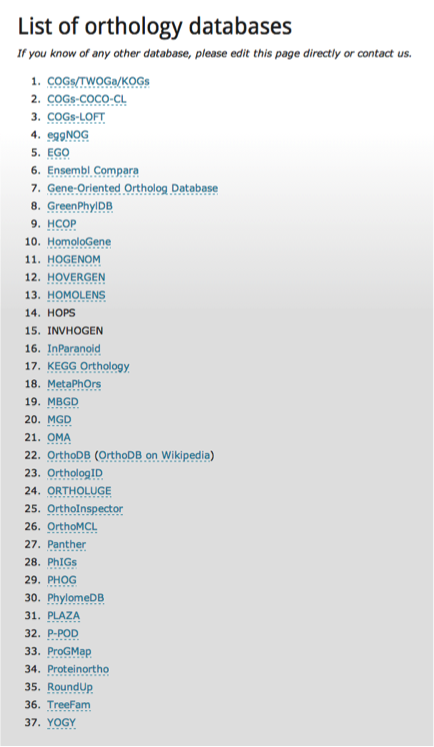
\includegraphics[height=0.575\textheight]{images/orthology_databases}      
    \end{column}
  \end{columns}
\end{frame}

% Which methods work best
\begin{frame}
  \frametitle{Reciprocal Best BLAST Hits
    \footnote{\tiny\href{http://armchairbiology.blogspot.co.uk/2012/07/on-reciprocal-best-blast-hits.html}{On Reciprocal Best BLAST Hits 19/7/2012
    }}
  }
  \begin{center}
      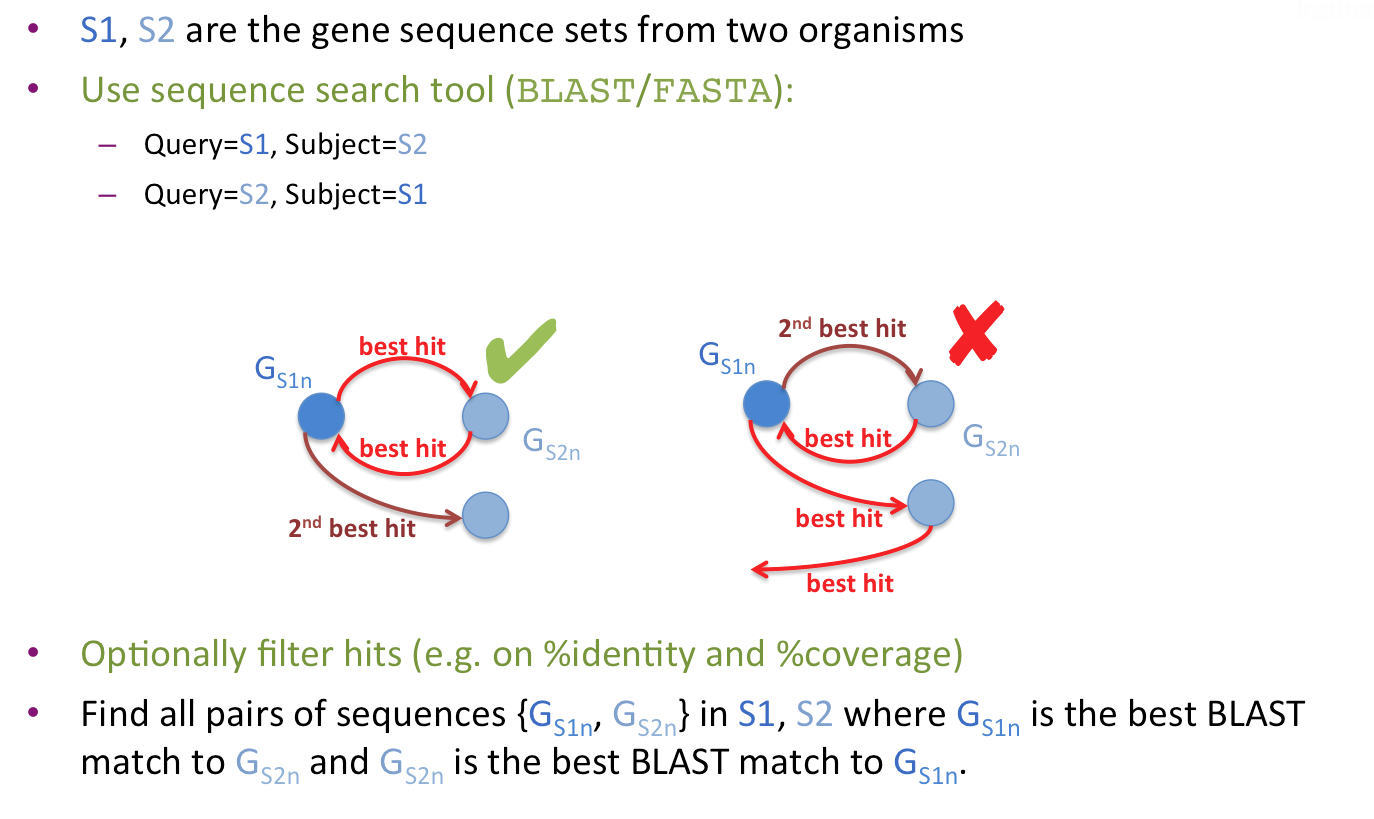
\includegraphics[width=1\textwidth]{images/rbbh}      
  \end{center}
\end{frame}

% 
\begin{frame}
  \frametitle{MCL
    \footnote{\tiny{Enright \textit{et al.} (2002) \textit{Nucl. Acids Res.} \href{http://dx.doi.org/10.1093/nar/30.7.1575}{doi:10.1093/nar/30.7.1575
    }}}
  }
  \begin{itemize}
    \item MCL constructs a network (\textit{graph}) from all-against-all BLAST results
    \item \textcolor{hutton_green}{Matrix operations (\textit{expansion}, \textit{inflation}) are applied}
    \item \textcolor{hutton_blue}{Expansion, inflation iterated until the network converges}
  \end{itemize}
  \begin{center}
      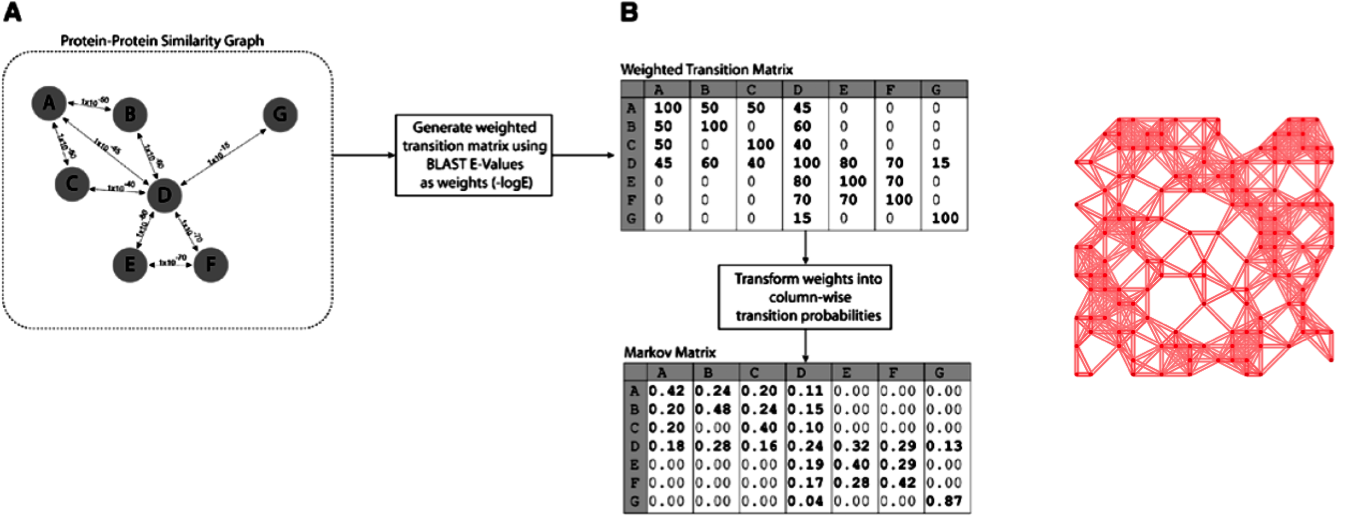
\includegraphics[width=1\textwidth]{images/mcl_intro}
  \end{center}
\end{frame}

% 
\begin{frame}
  \frametitle{MCL
    \footnote{\tiny{Enright \textit{et al.} (2002) \textit{Nucl. Acids Res.} \href{http://dx.doi.org/10.1093/nar/30.7.1575}{doi:10.1093/nar/30.7.1575
    }}}
  }  
  \begin{center}
      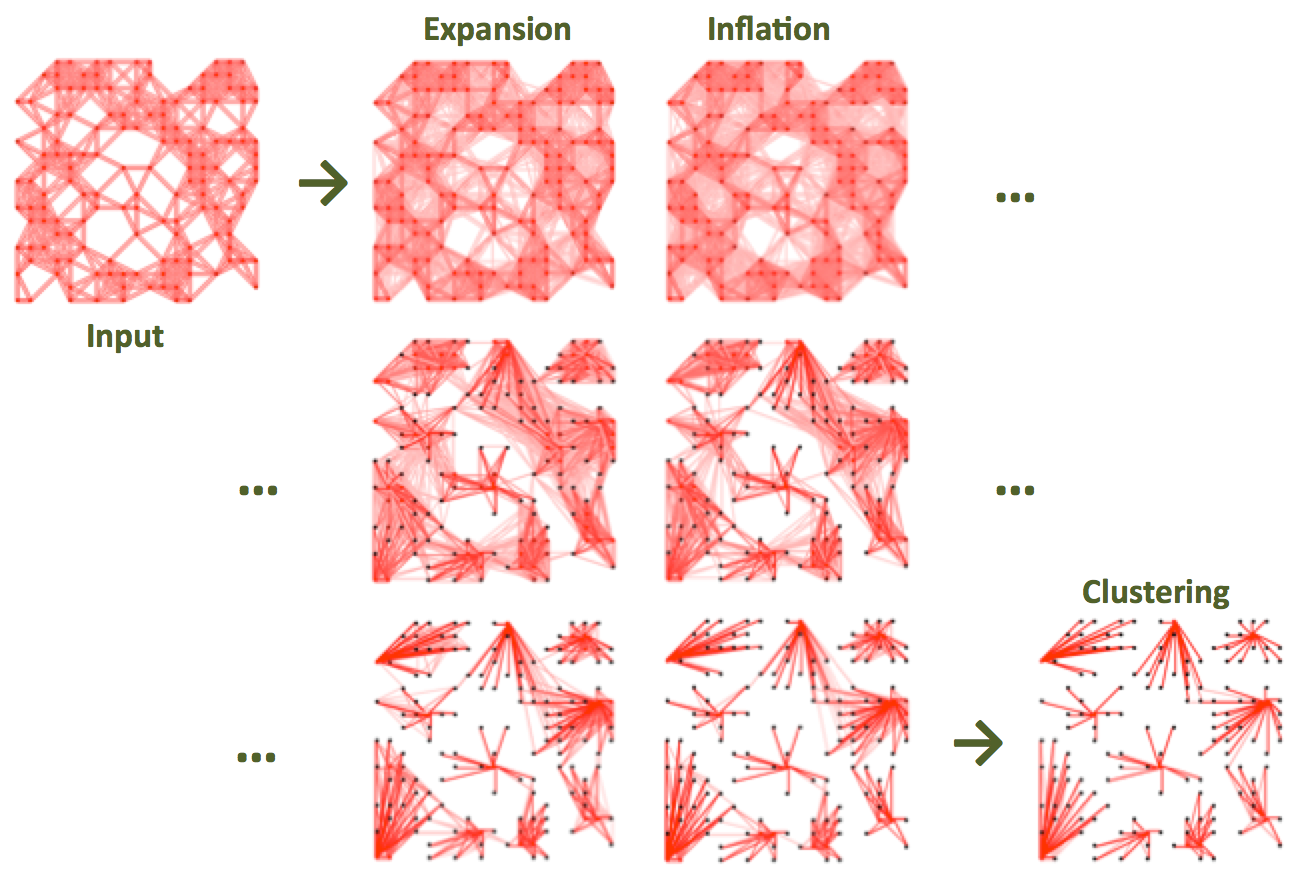
\includegraphics[width=1\textwidth]{images/mcl_method}
  \end{center}
\end{frame}

% 
\begin{frame}
  \frametitle{Which prediction methods work best?
    \footnote{\tiny{Salichos and Rokas (2011) \textit{PLoS One} \textbf{6}:e18755 \href{http://dx.doi.org/10.1371/journal.pone.0018755.g006}{doi:10.1371/journal.pone.0018755.g006
  }}}
  }
  Four methods tested against 2,723 curated orthologues from six \textit{Saccharomycetes}
  \begin{itemize}
    \item \textcolor{hutton_green}{RBBH (and cRBH); RSD (and cRSD); MultiParanoid; OrthoMCL}
    \item \textcolor{hutton_blue}{Rated by statistical performance metrics: sensitivity, specificity, accuracy, FDR}
  \end{itemize}
  \textcolor{hutton_purple}{\textbf{cRBH most accurate and specific, with lowest FDR.}}
  \begin{center}
      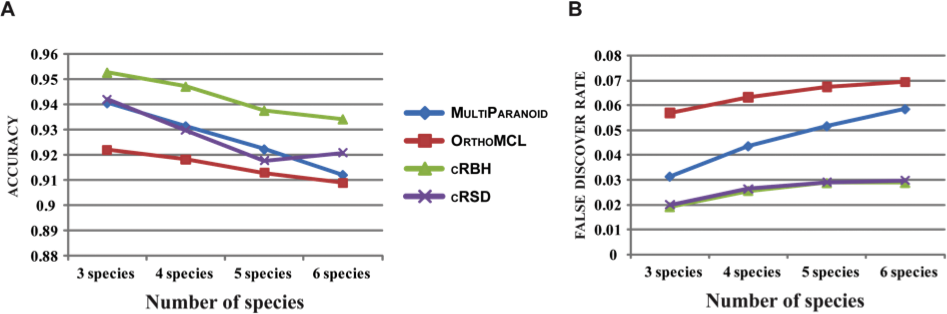
\includegraphics[height=0.25\textheight]{images/salichos_results1} 
      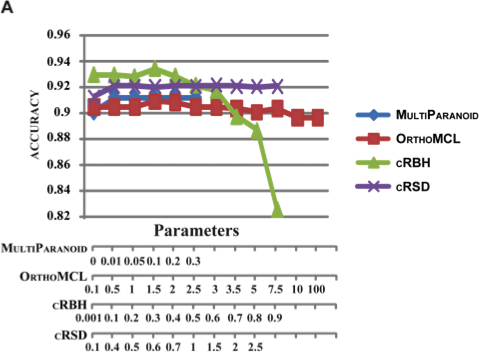
\includegraphics[height=0.25\textheight]{images/salichos_results2}      
  \end{center}
\end{frame}

% 
\begin{frame}
  \frametitle{Which prediction methods work best?
    \footnote{\tiny{Wolf and Koonin (2012) \textit{Genome Biol. Evol.} \textbf{4}:1286-1294 \href{http://dx.doi.org/10.1093/gbe/evs100}{doi:10.1093/gbe/evs100
    }}}
    \footnote{\tiny{Altenhoff and Dessimoz (2009) \textit{PLoS Comp. Biol.} \textbf{5}:e1000262 \href{http://dx.doi.org/10.1371/journal.pcbi.1000262}{doi:10.1371/journal.pcbi.1000262
    }}}
  }
  \begin{itemize}
    \item \textcolor{hutton_green}{Performance varies by choice of method, and interpretation of ``orthology''}
    \item \textcolor{hutton_blue}{Biggest influence is genome annotation quality}
    \item Relative performance varies with choice of benchmark
    \item \textcolor{hutton_purple}{\textbf{(clustering) RBH outperforms more complex algorithms under many circumstances}}
  \end{itemize}
\end{frame}

%
\begin{frame}
  \frametitle{How orthologues help}
  \textcolor{hutton_green}{Defining core groups of genes as ``orthologues'' allows analysis of groups of genes by:}
  \begin{itemize}
    \item \textcolor{hutton_purple}{synteny/collocation}
    \item gene neighbourhood changes (e.g. \textcolor{hutton_purple}{\textit{genome expansion}})
    \item \textcolor{hutton_purple}{pan genome (core/accessory genomes)}
  \end{itemize}
  \textcolor{hutton_blue}{and of individual genes within those groups, by:}
  \begin{itemize}
    \item multiple alignment
    \item domain detection
    \item identification of functional sites
    \item inference of directional selection (stabilising/positive selection)
  \end{itemize}  
\end{frame}

%
\begin{frame}
  \frametitle{Genome expansion
    \footnote{\tiny{Haas \textit{et al}. (2009) \textit{Nature} \href{http://dx.doi.org/10.1038/nature08358
}{doi:10.1038/nature08358
  }}}
}
  \begin{itemize}
    \item \textcolor{hutton_green}{Mobile/repeat elements reproduce and expand during evolution} 
    \item \textcolor{hutton_blue}{Generates a ``sequence laboratory'' for variation and experiment}
    \item \textcolor{RawSienna}{e.g. \textit{Phytophthora infestans} effector protein expansion and arms race}
  \end{itemize}  
    \begin{center}
      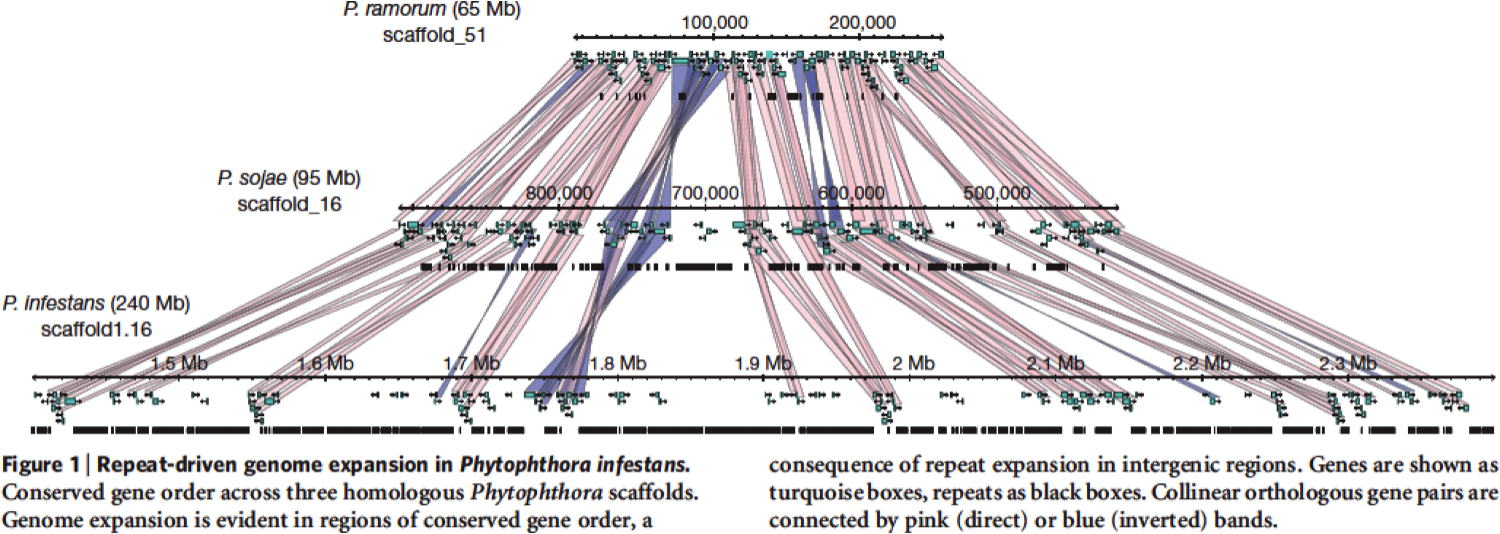
\includegraphics[width=\textwidth]{images/pi_expansion}      
    \end{center}    
\end{frame}

%
\begin{frame}
  \frametitle{Genome expansion
    \footnote{\tiny{Haas \textit{et al}. (2009) \textit{Nature} \href{http://dx.doi.org/10.1038/nature08358
}{doi:10.1038/nature08358
  }}}
}
  \begin{columns}[T] 
    \column{.4\textwidth}   
      \begin{itemize}
        \item Mobile elements (MEs) are large, and duplicate/carry genes with them
        \item \textcolor{hutton_green}{Larger intergenic regions in MEs}
        \item \textcolor{hutton_blue}{Effector proteins found preferentially in regions with large gaps}
        \item \textcolor{hutton_purple}{Two-speed genome associated with adaptability}
      \end{itemize}  
      \column{.6\textwidth}
        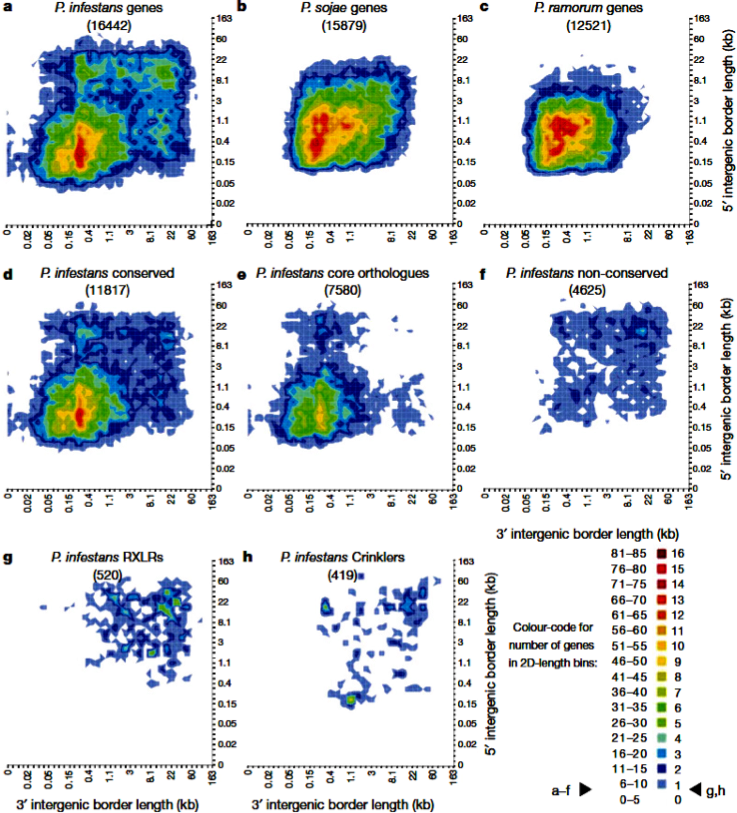
\includegraphics[width=\textwidth]{images/pi_two_speed}
    \end{columns}
\end{frame}

%
\begin{frame}
  \frametitle{The Pangenome
  }
  \Large{
    \textcolor{olive}{
      \textbf{
      The Core Genome Hypothesis: \\
      ``The \textit{core genome} is the primary cohesive unit defining a bacterial species''
      }
    }
  }
\end{frame}

% Which methods work best
\begin{frame}
  \frametitle{Core genome   
  \footnote{\tiny{Laing (2010) \textit{BMC Bioinf.} \href{http://dx.doi.org/10.1186/1471-2105-11-461}{doi:10.1186/1471-2105-11-461
  }}}
    \footnote{\tiny{Lef\'{e}bure \textit{et al}. (2010) \textit{Genome Biol. Evol.} \href{http://dx.doi.org/10.1371/10.1093/gbe/evq048}{doi:10.1093/gbe/evq048
    }}}  
}
  \textcolor{hutton_green}{Once equivalent genes have been identified, those present in all related isolates can be identified: \textbf{\textit{the core genome}}.}\\
  \begin{center}
      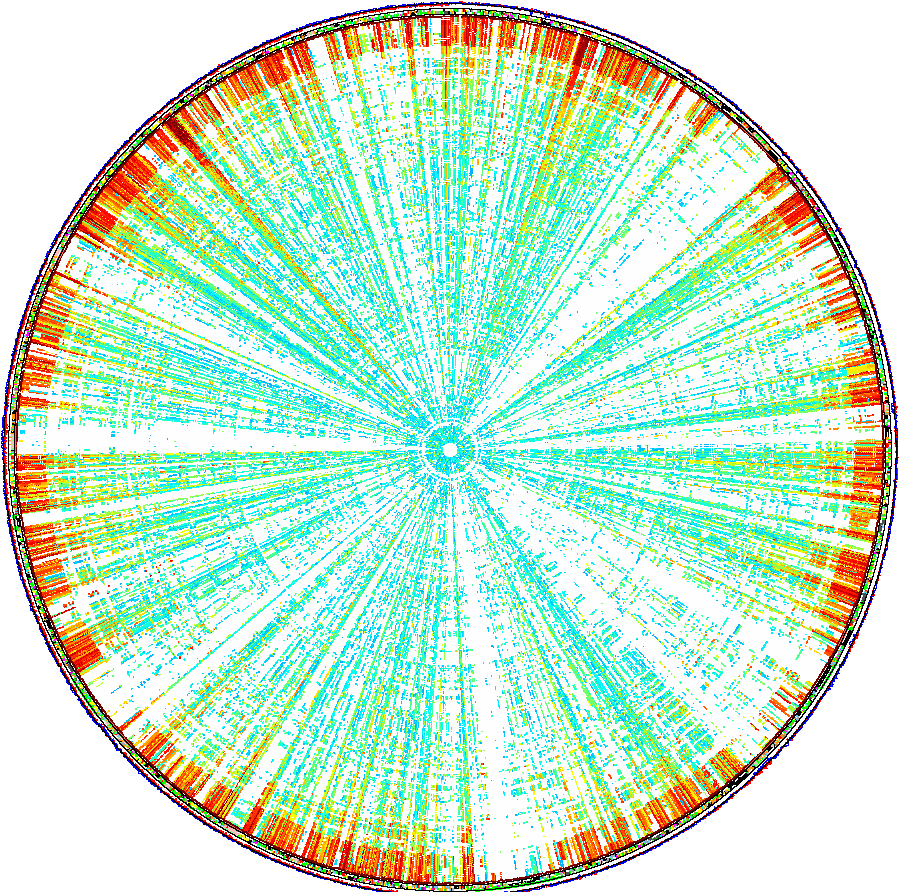
\includegraphics[height=0.5\textheight]{images/pba_400_circular}
      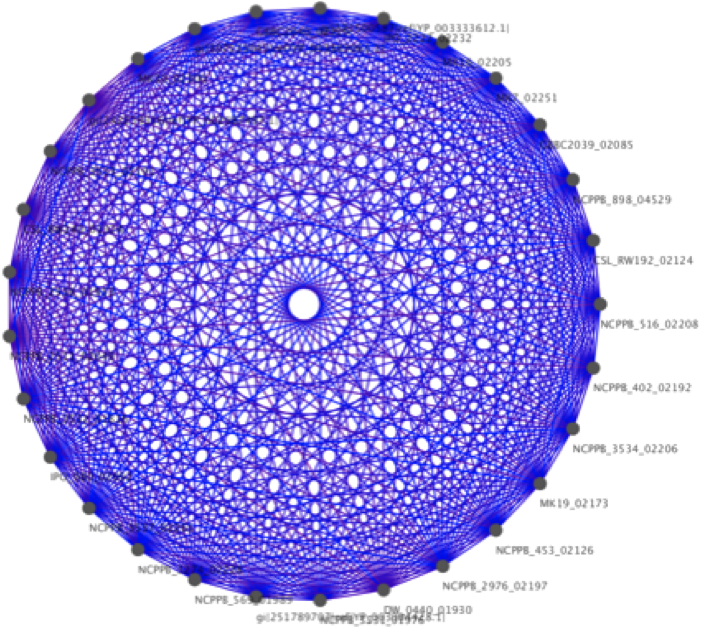
\includegraphics[height=0.5\textheight]{images/core_cluster}      
  \end{center}
\end{frame}

% Which methods work best
\begin{frame}
  \frametitle{Accessory genome
    \footnote{\tiny{Laing (2010) \textit{BMC Bioinf.} \href{http://dx.doi.org/10.1186/1471-2105-11-461}{doi:10.1186/1471-2105-11-461
  }}}
    \footnote{\tiny{Lef\'{e}bure \textit{et al}. (2010) \textit{Genome Biol. Evol.} \href{http://dx.doi.org/10.1371/10.1093/gbe/evq048}{doi:10.1093/gbe/evq048
    }}}  
}
  \textcolor{hutton_green}{The remaining genes are \textbf{\textit{the accessory genome}}, and are expected to mediate function that distinguishes between isolates.}\\[0.2cm]
  \begin{center}
      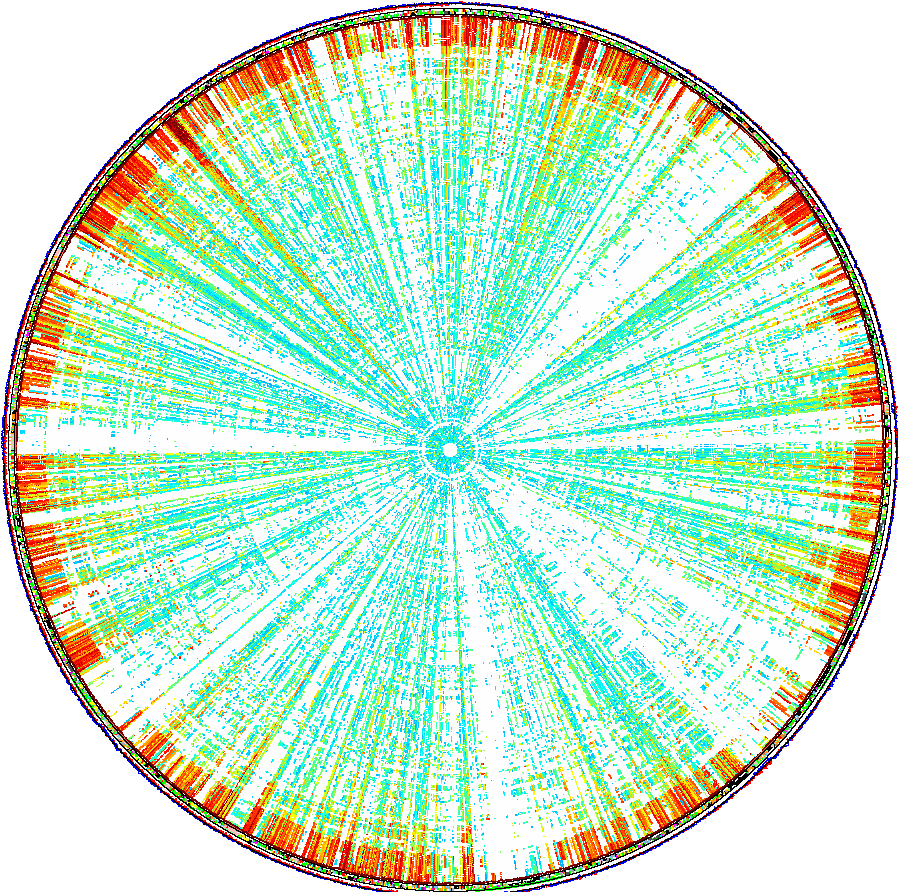
\includegraphics[height=0.5\textheight]{images/pba_400_circular}        
      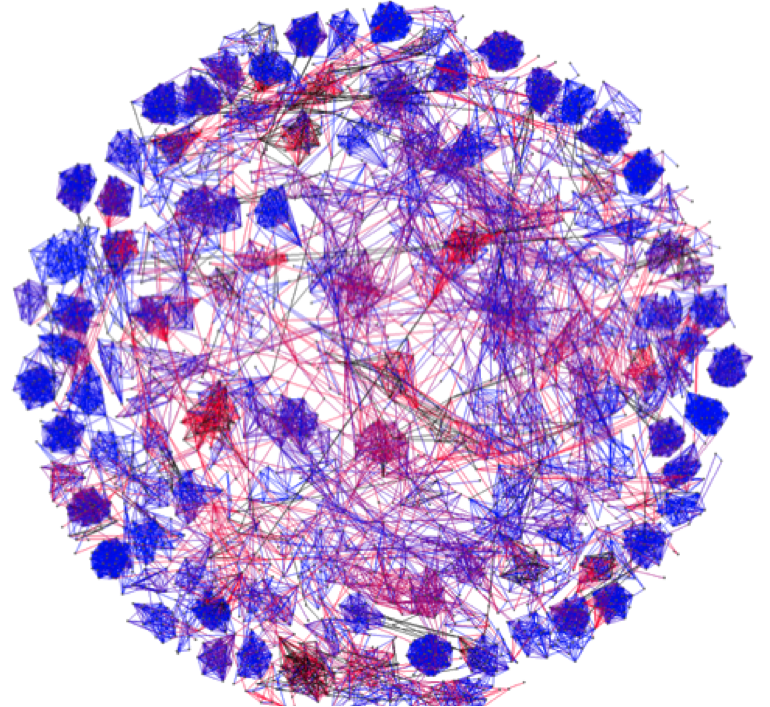
\includegraphics[height=0.5\textheight]{images/accessory_cluster}      
  \end{center}
\end{frame}

% Which methods work best
\begin{frame}
  \frametitle{Accessory genome
   \footnote{\tiny{Croll and Mcdonald (2012) \textit{PLoS Path.} \textbf{8}:e1002608 \href{http://dx.doi.org/10.1371/journal.ppat.1002608}{doi:10.1371/journal.ppat.1002608
  }}}
    \footnote{\tiny{Baltrus \textit{et al}. (2011) \textit{PLoS Path.} \textbf{7}:e1002132 \href{http://dx.doi.org/10.1371/journal.ppat.1002132}{doi:10.1371/journal.ppat.1002132.t002
    }}}  
  }
  Accessory genomes are a cradle for adaptive evolution \\
  \textcolor{hutton_green}{This is particularly so for bacterial pathogens, such as \textit{Pseudomonas} spp.}
  \begin{center}
      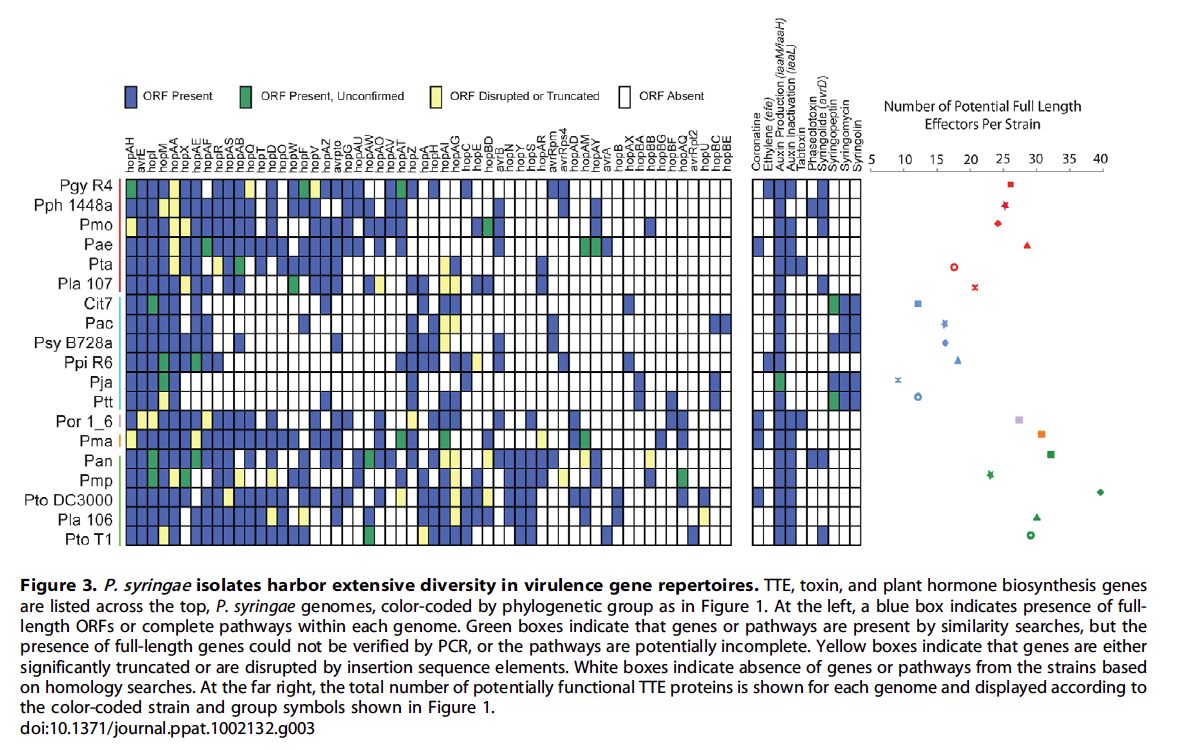
\includegraphics[height=0.5\textheight]{images/pa_virulence} 
  \end{center}
\end{frame}

% Which methods work best
\begin{frame}
  \frametitle{Identifying the Pangenome
   \footnote{\tiny{Page \textit{et al.} (2015) \textit{Bioinf.} \textbf{31}:3691-3693 \href{http://dx.doi.org/10.1093/bioinformatics/btv421}{doi:10.1093/bioinformatics/btv421
  }}}
  }
  \texttt{Roary} can produce pangenomes for 1000s of prokaryotes on a desktop machine
  \begin{columns}[T] 
    \column{.4\textwidth}   
      \begin{itemize}
        \item \textcolor{hutton_green}{Pre-cluster with CD-HIT (reduce input size)}
        \item \textcolor{hutton_blue}{All-against-all on reduced sequence set}
        \item \textcolor{hutton_purple}{MCL clustering}
        \item \textcolor{RawSienna}{Merge clusters and use synteny to identify orthologues}        
      \end{itemize}  
      \column{.6\textwidth}
        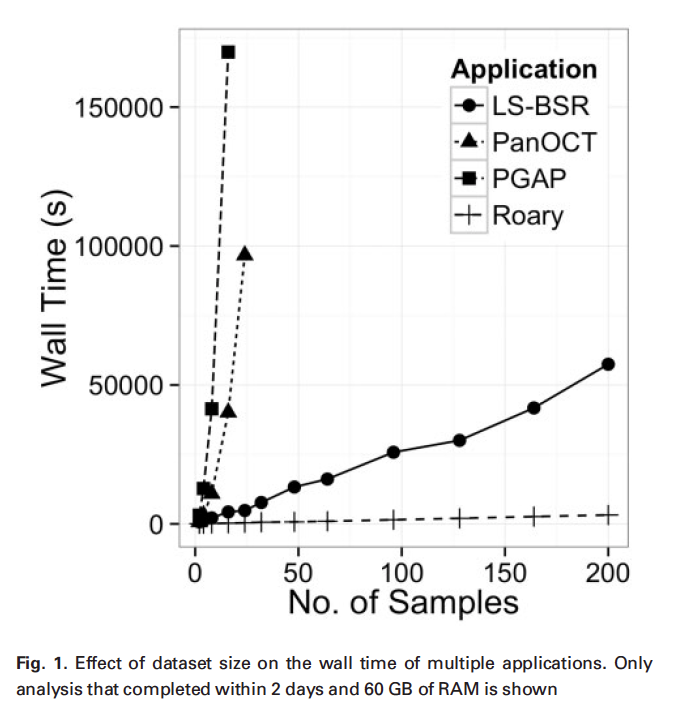
\includegraphics[width=0.8\textwidth]{images/roary_performance}
    \end{columns}  
  \end{frame}

%
\begin{frame}
  \frametitle{What didn't I get to?}
  \begin{itemize}
    \item   \textcolor{hutton_green}{Genome-Wide Association Studies (GWAS)}
    \begin{itemize}
      \item   Try \href{http://genenetwork.org/}{http://genenetwork.org/} to play with some data
    \end{itemize}
    \item Prediction of regulatory elements, e.g.
    \begin{itemize}
      \item {\tiny\href{http://dx.doi.org/10.1038/nature01644}
                              {Kellis \textit{et al.} (2003) \textit{Nature} doi:10.1038/nature01644}}
      \item {\tiny\href{http://dx.doi.org/10.1101/gr.5592107}
                              {King \textit{et al.} (2007) \textit{Genome Res.} doi:10.1101/gr.5592107}}
      \item {\tiny\href{http://dx.doi.org/10.1186/1471-2105-9-455}
                              {Chaivorapol \textit{et al.} (2008) \textit{BMC Bioinf.} doi:10.1186/1471-2105-9-455}}
      \item {\tiny\href{http://genome.ucsf.edu/compmoby}
                              {CompMOBY http://genome.ucsf.edu/compmoby}}
    \end{itemize}
    \item   \textcolor{hutton_purple}{Detection of Horizontal/Lateral Gene Transfer (HGT/LGT), e.g.}
    \begin{itemize}
      \item {\tiny\href{http://dx.doi.org/10.1093/nar/gki187}
                              {Tsirigos \& Rigoutsos (2005) \textit{Nucl. Acids Res.} doi:10.1093/nar/gki187}}
    \end{itemize}
    \item   \textcolor{RawSienna}{Phylogenomics, e.g.}
    \begin{itemize}
      \item {\tiny\href{http://dx.doi.org/10.1038/nrg1603}
                              {Delsuc \textit{et al.} (2005) \textit{Nat. rev. Genet.} doi:10.1038/nrg1603}}
      \item {\tiny\href{https://phylogenomics.wordpress.com/software/amphora/}
                              {AMPHORA https://phylogenomics.wordpress.com/software/amphora/}}
    \end{itemize}
  \end{itemize}
\end{frame}

\begin{frame}
  \frametitle{Messages to take away}
  \begin{itemize}
    \item   \textcolor{hutton_green}{Comparative genomics is a powerful set of techniques for:}
    \begin{itemize}
      \item Understanding and identifying evolutionary processes and mechanisms
      \item Reconstructing detailed evolutionary history
      \item Identifying and understanding common genomic features
      \item Providing hypotheses about gene function for experimental investigation
    \end{itemize}
  \end{itemize}
\end{frame}

\begin{frame}
  \frametitle{Messages to take away}
  \begin{itemize}
    \item \textcolor{hutton_green}{Comparative genomics is comparisons}
    \begin{itemize}
      \item What is \textit{similar} between two genomes?
      \item What is \textit{different} between two genomes?
    \end{itemize}
    \item \textcolor{hutton_blue}{Comparative genomics \textit{is} evolutionary genomics}
    \begin{itemize}
      \item Lots of scope for improvement in tools
    \end{itemize}
    \item \textcolor{hutton_purple}{Tools that `do the same thing' can give different output}
    \begin{itemize}
      \item BLAST vs MUMmer
      \item RBBH vs MCL
      \item The choice of application matters for correctness and interpretation
    \end{itemize}
  \end{itemize}
\end{frame}
